\documentclass[spanish]{beamer}
\usepackage[ansinew]{inputenc} % Acepta caracteres en castellano
\usepackage[spanish]{babel}    % silabea palabras castellanas
\usepackage{amsmath}
\usepackage{mathtools,cancel} % cancela con una flecha \cancelto{0}{XXXX}
\renewcommand{\CancelColor}{\color{red}} %change cancel color to red
\usepackage{amsfonts}
\usepackage{amssymb}
\usepackage{dsfont}
\usepackage{graphicx}
\usepackage{geometry}
\usetheme{Madrid}
\usecolortheme{beaver}
\usepackage{textpos}
% Logo  en el comienzo 
\addtobeamertemplate{frametitle}{}{%
\begin{textblock*}{100mm}(.85\textwidth,-1cm)
{\includegraphics[height=0.4in, keepaspectratio=true]{/Users/luisnunez/Dropbox/MisDocumentos/UIS/UISImagenInstitucional/UISLOGO.png}}
\end{textblock*}}

\begin{document}

\title{\textbf{Hamilton Jacobi} }
\author[L.A. N��ez]{\textbf{Luis A. N��ez}}  
\institute[UIS]{\textit{Escuela de F�sica, Facultad de Ciencias, } \\
\textit{Universidad Industrial de Santander, Santander, Colombia } \\
{\includegraphics[height=0.4in, keepaspectratio=true]{/Users/luisnunez/Dropbox/MisDocumentos/UIS/UISImagenInstitucional/UISLOGO.png}}
}
\date{\today}
\maketitle


\begin{frame}
\frametitle{Agenda}
  \tableofcontents
\end{frame}


%%%%% Diapo 1
\section{Ecuaci�n de Hamilton Jacobi}
\frame{
  \frametitle{Ecuaci�n de Hamilton Jacobi}
   \begin{itemize}  
  	\item<1-> Una transformaci�n can�nica $Q_i=Q_i\left(q_j, p_j, t\right), P_i=P_i\left(q_j, p_j, t\right)$, permite encontrar las soluciones de las ecuaciones de Hamilton.
	\item<2-> Esa transformaci�n $Q_i=Q_i\left(q_j, p_j, t\right), P_i=P_i\left(q_j, p_j, t\right)$ lleva $\mathcal{H}\left(q_j, p_j, t\right)\rightarrow \mathcal{H}^{\prime}\left(Q_i, P_i, t\right)$ un hamiltoniano en el cual una (o varias) coordenada $Q_j$ o/y $P_j$ son c�clicas
	\item<3-> Supongamos una transformaci�n can�nica $\left\{q_i, p_i, t\right\} \rightarrow \left\{P_i, Q_i, t\right\}$ tal que, $\left(P_i, Q_i\right)$, las $2 s$ nuevas coordenadas y momentos  son constantes.
	\item<4-> Esas $2 s$ constantes $Q_i$ y $P_i$ pueden expresarse en funci�n de las $2 s$ condiciones iniciales:  $Q_i=q\left(q_j(0), p_j(0)\right), P_i=p\left(q_j(0), p_j(0)\right)$.
	\item<5-> La transformaci�n can�nica que relacionan las nuevas y viejas variables proporcionan directamente la soluci�n del problema del movimiento, $q_i=q\left(q_j(0), p_j(0), t\right), \quad p_i=p\left(q_j(0), p_j(0), t\right)$.
	\item<6-> Si  la transformaci�n can�nica conduce a nuevos momentos y coordenadas constantes, $P_i \equiv \alpha_i=$ cte, $Q_i \equiv \beta_i=$ cte, tal que $\mathcal{H}^{\prime}\left(Q_i, P_i\right)=0$, entonces existe una funci�n generadora $\mathcal{F}$ tal que $\frac{\partial F}{\partial t}+H=0$
	\item<7-> Esta condici�n es la ecuaci�n de Hamilton-Jacobi, para una $\mathcal{F}$.
    \end{itemize}
}
%
%%%%% Diapo 2
\section{Hamilton-Jacobi y el Principio de M�nima Acci�n}
\frame{
\frametitle{El Principio de M�nima Acci�n 1/2}
\begin{itemize}  
	\item<1-> Consideremos la acci�n $S=\int_{t_1}^{t_2} L\left(q_i, \dot{q}_i, t\right) d t $
	\item<2-> El valor de la acci�n $S$ (como integral definida) depende del conjunto de trayectorias $\left\{q_i(t)\right\}$
	\item<3-> Las trayectorias que satisfacen la ecuaciones de Lagrange corresponden al valor m�nimo (extremo) de $S$.
	\item<4-> Supongamos que el tiempo $t_2$ es variable, i.e, $t_2=t$.
	\item<5-> La acci�n depender� de las trayectorias y del tiempo, $S=S\left(q_i, t\right)$.
	\begin{figure}[t]
		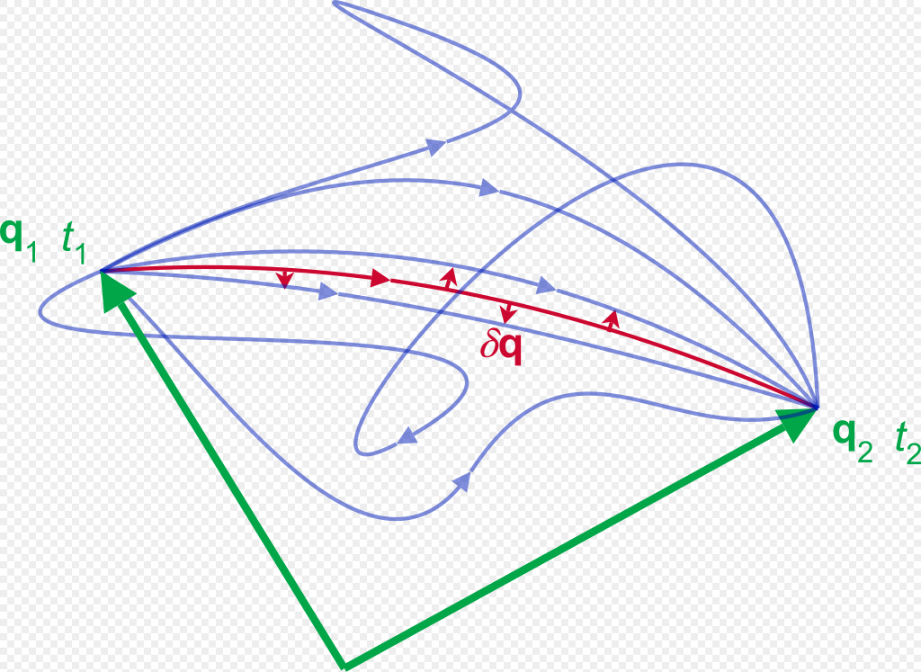
\includegraphics[width=1.5in]{Figuras/Trayectorias1.png}
		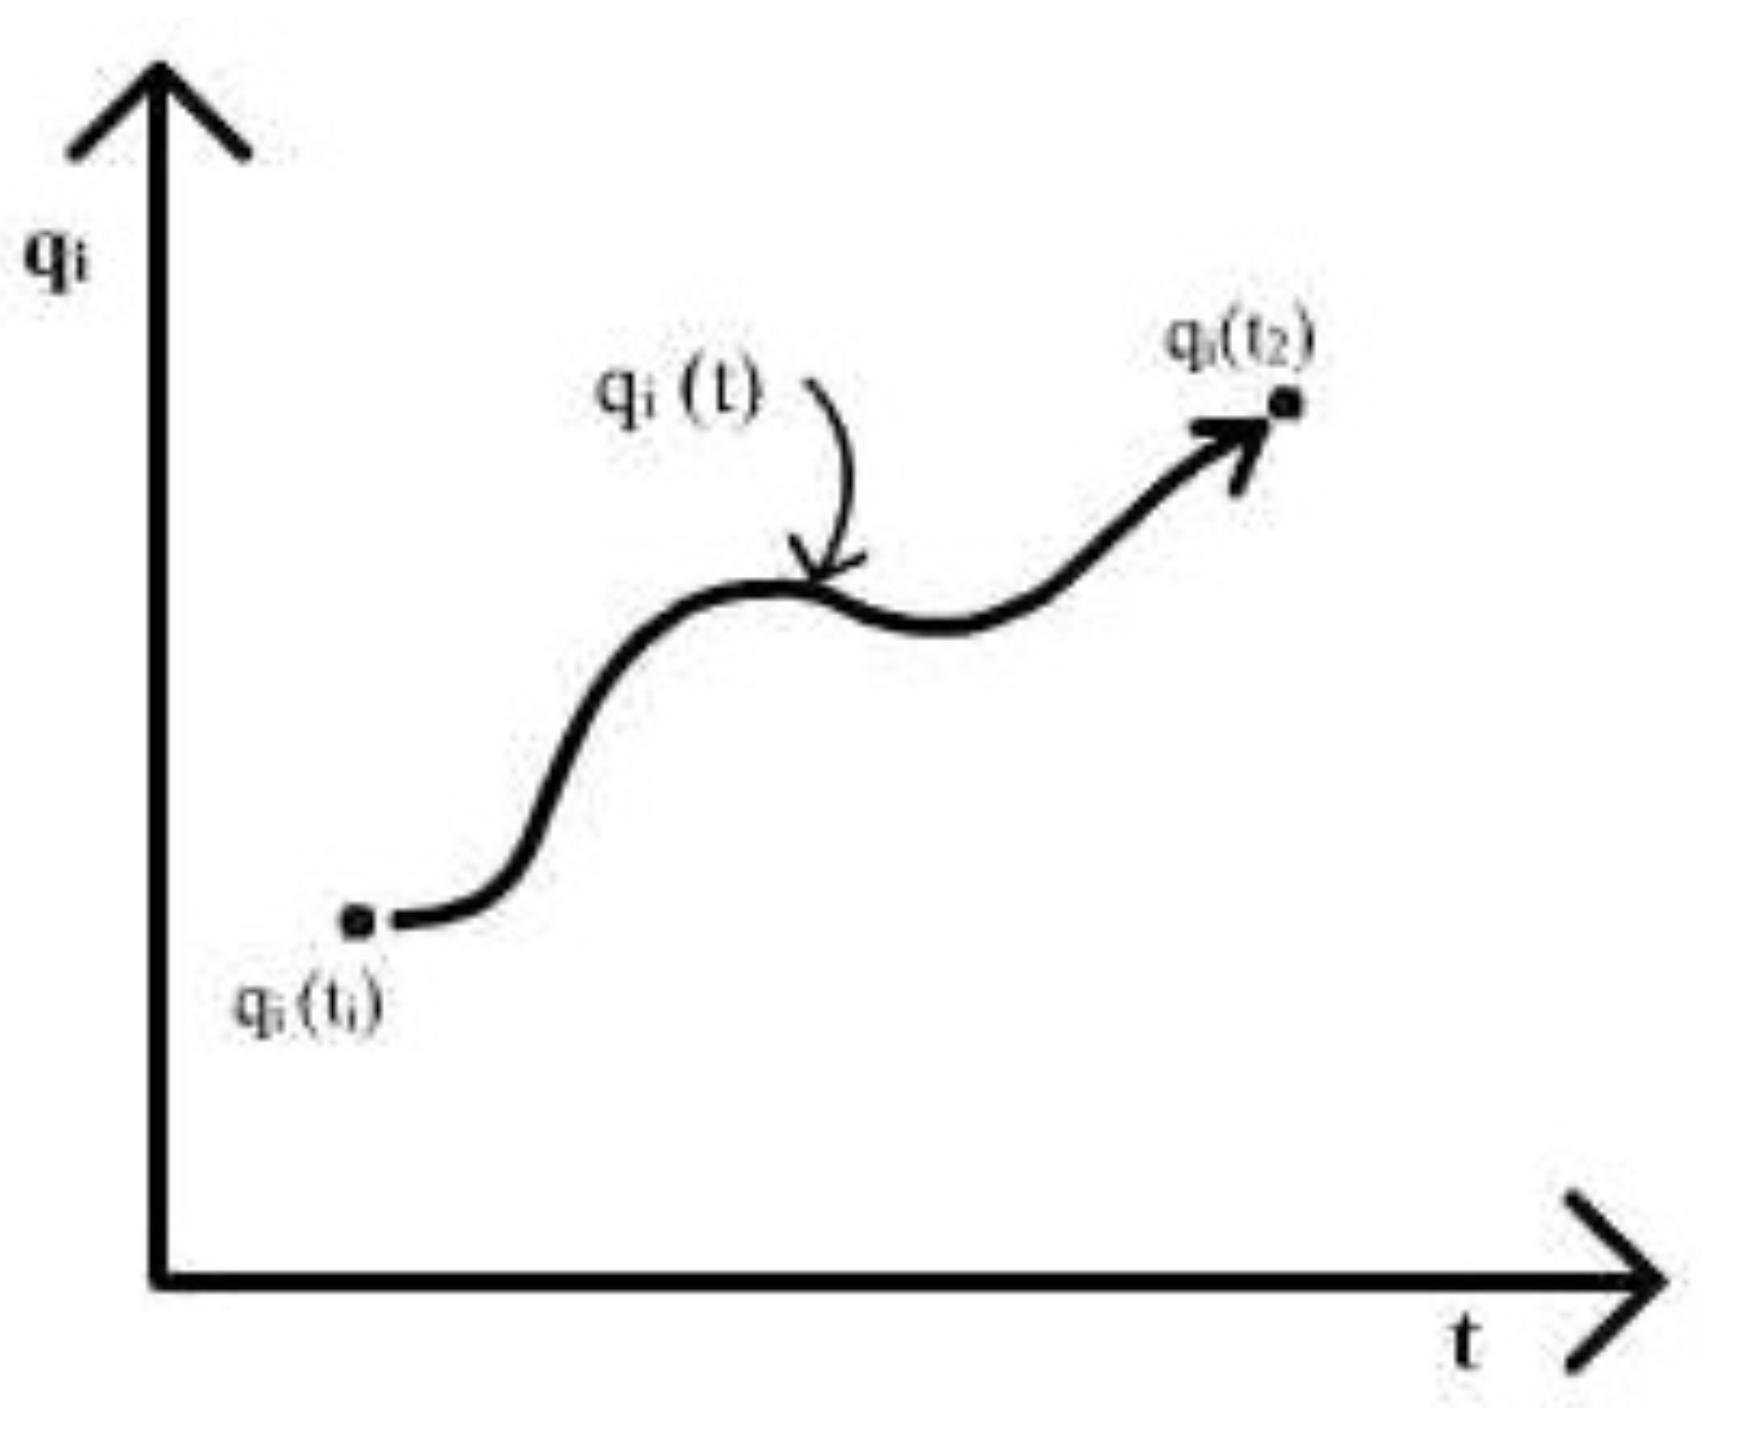
\includegraphics[width=1.5in]{Figuras/Trayectorias2.png}
   	\end{figure}
\end{itemize}
}
%
%%%%% Diapo 2
%\section{Secci�n}
\frame{
\frametitle{El Principio de M�nima Acci�n 2/2}
\begin{itemize}  
	\item<1-> La derivada temporal de la acci�n es $\frac{d S}{d t}=\sum_{i=1}^s \frac{\partial S}{\partial q_i} \dot{q}_i+\frac{\partial S}{\partial t}$.	
	\item<2-> Por otro lado, si $t_2=t$ (variable), la definici�n de la acci�n implica que $\frac{d S}{d t}=\mathcal{L}=\sum_{i=1}^s p_i \dot{q}_i-H\left(p_i, q_i, t\right)$.
	\item<3-> Comparando obtenemos $ p_i=\frac{\partial S}{\partial q_i}\left(q_i, t\right)$ y $\frac{\partial S}{\partial t}\left(q_i, t\right)+\mathcal{H}\left(p_i, q_i, t\right)=0$
	\item<4-> Las cuales se pueden expresar como $\frac{\partial S}{\partial t}\left(q_i, t\right)+\mathcal{H}\left(\frac{\partial S}{\partial q_i}, q_i, t\right)=0$
	\item<5-> La acci�n $S$ puede interpretarse como una funci�n generadora capaz de producir la transformaci�n can�nica.
	\item<6-> M�s a�n, la acci�n $S$ puede interpretarse como una funci�n generadora tipo $\mathcal{F}_2\left(q_i, P_i, t\right)$, tal que $P_i=\alpha_i=$ cte, $Q_i=\beta_i=$ cte.
\end{itemize}
}
  
\end{document}
%
%%%%% Diapo 2
\section{Secci�n}
\frame{
\frametitle{T�tulo transparencia}
\begin{itemize}  
	\item<1-> 
\end{itemize}
}

	\begin{figure}[t]
		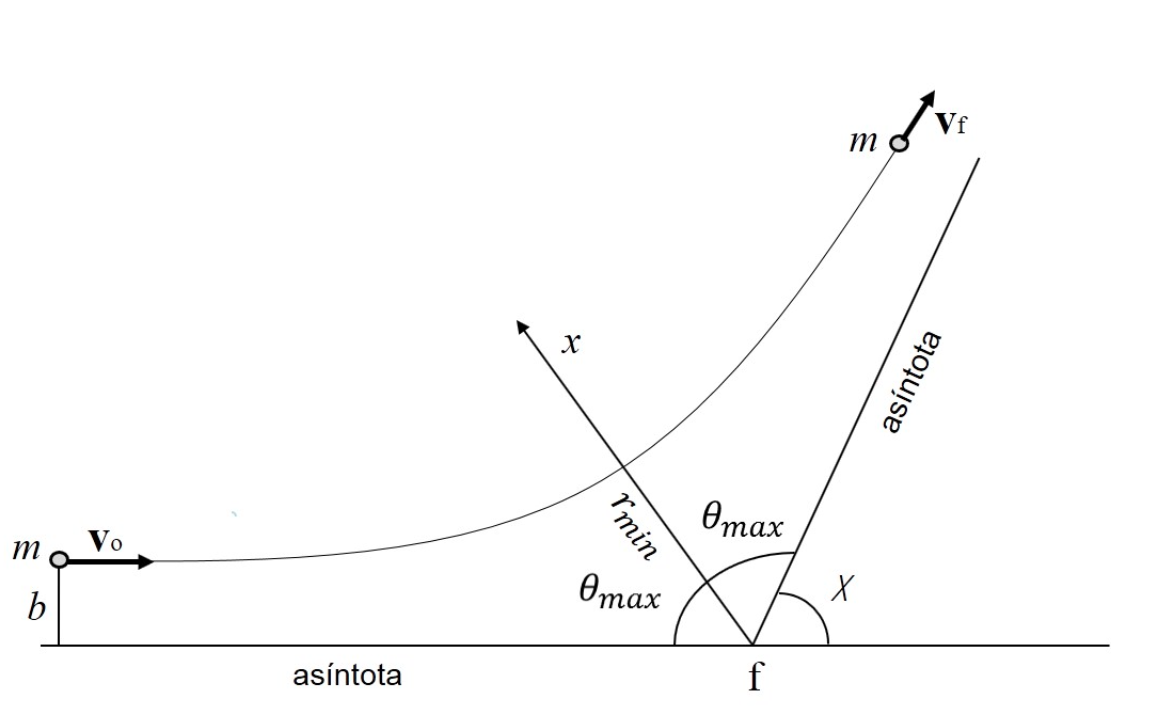
\includegraphics[width=1.8in]{Figuras/Dispersion.png}
   	\end{figure}
	
